\begin{activity} \label{A:9.1.6}
    In the following questions, we investigate the use of traces to better understand a function through both tables and graphs.  
    \ba
  \item Identify the $y = 0.6$ trace for the range function $f(x,y) =
    \frac{x^2 \sin(2y)}{g}$ by highlighting or circling the
    appropriate cells in Table \ref{T:9.1.range}.  Write a sentence to
    describe the behavior of the function along this trace.

  \item Identify the $x = 150$ trace for the range function by
    highlighting or circling the appropriate cells in Table
    \ref{T:9.1.range}.  Write a sentence to describe the behavior of
    the function along this trace.

 \begin{figure}[ht]
\begin{center}
%\resizebox{!}{2.0in}{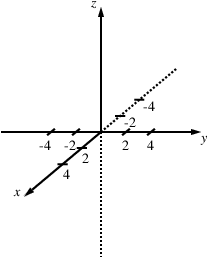
\includegraphics{figures/9_1_traces_activity_1}}
  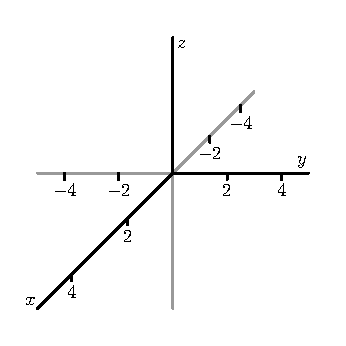
\includegraphics{figures/fig_9_1_activity_axes.eps}
\caption{Coordinate axes to sketch traces.}
\label{F:9.1.traces_activity_1}
\end{center}
\end{figure}

   \item For the function $g(x,y) = x^2 + y^2 + 1$, explain the type of function that each trace in the $x$ direction will be (keeping $y$ constant). Plot the $y=-4$, $y=-2$, $y=0$, $y=2$, and $y=4$ traces in 3-dimensional coordinate system provided in Figure \ref{F:9.1.traces_activity_1}.

    \item For the function $g(x,y) = x^2 + y^2 + 1$, explain the type of function that each trace in the $y$ direction will be (keeping $x$ constant). Plot the $x=-4$, $x=-2$, $x=0$, $x=2$, and $x=4$ traces in 3-dimensional coordinate system in Figure \ref{F:9.1.traces_activity_1}.

    \item Describe the surface generated by the function $g$.

     \ea



\end{activity}
\begin{smallhint}
\ba
\item Do the $y$ values run down the columns or across the rows?
\item Do the $x$ values run down the columns or across the rows?
\item If $y$ is constant, the only variables are $x$ and $z$. 
\item If $x$ is constant, the only variables are $y$ and $z$.
\item What do the traces look like?
\ea 
\end{smallhint}
\begin{bighint}
\ba
\item Do the $y$ values run down the columns or across the rows?
\item Do the $x$ values run down the columns or across the rows?
\item What does the graph of $z=x^2+C$ look like if $C$ is a constant?
\item What does the graph of $z=y^2+C$ look like if $C$ is a constant?
\item What do the traces look like?
\ea
\end{bighint}
\begin{activitySolution}
\ba
\item The $y$ values in the table are those that run across the rows. So fixing $y$ at $\frac{2\pi}{5} = \frac{8\pi}{20}$ and letting $x$ vary amounts to looking at the $\frac{8\pi}{20}$ column in the table. The $y=\frac{2\pi}{5}$ trace is highlighted in red in the table below. This trace shows that as we increase the initial velocity $x$ while keeping the launch angle constant at $\frac{2\pi}{5}$ radians, the range of the object increases at an increasing rate. 
\begin{center}
\begin{tabular}{|c|c|c|c|c|c|c|c|>{\columncolor{tracered}}c|c|c|} \hline
  &$\frac{\pi}{20}$ &$\frac{2\pi}{20}$ &$\frac{3\pi}{20}$ &$\frac{4\pi}{20}$ &$\frac{5\pi}{20}$ &$\frac{6\pi}{20}$ &$\frac{7\pi}{20}$ &$\frac{8\pi}{20}$ &$\frac{9\pi}{20}$    &$\frac{\pi}{2}$ \\ \hline
25      &6.036      &11.480     &15.801     &18.575     &19.531     &18.575     &15.801     &11.480     &6.0356     &0.000 \\ \hline
50      &24.142     &45.921     &63.205     &74.301     &78.125     &74.301     &63.205     &45.921     &24.142     &0.000 \\ \hline
75      &54.319     &103.322    &142.210    &167.178    &175.781    &167.178    &142.210    &103.322    &54.319     &0.000 \\ \hline
100     &96.568     &183.683    &252.818    &297.205    &312.500    &297.205    &252.818    &183.683    &96.568     &0.000 \\ \hline
125     &150.887    &287.005    &395.028    &464.383    &488.281    &464.383    &395.028    &287.005    &150.887    &0.000 \\ \hline
150     &217.278    &413.287    &568.840    &668.712    &703.125    &668.712    &568.840    &413.287    &217.278    &0.000 \\ \hline
175     &295.739    &562.529    &774.255    &910.191    &957.031    &910.191    &774.255    &562.529    &295.739    &0.000 \\ \hline
200     &386.271    &734.732    &1011.271   &1188.821   &1250.000   &1188.821   &1011.271   &734.732    &386.271    &0.000 \\ \hline
225     &488.875    &929.895    &1279.890   &1504.601   &1582.031   &1504.601   &1279.890   &929.895    &488.875    &0.000 \\ \hline
250     &603.549    &1148.018   &1580.112   &1857.532   &1953.125   &1857.532   &1580.112   &1148.018   &603.549    &0.000 \\ \hline
\end{tabular}
\end{center}
\item  The $x$ values in the table are those that run down the columns. So fixing $x$ at $150$ and letting $y$ vary amounts to looking at the $150$ row in the table. The $x=150$ trace is highlighted in blue in the table below. This trace shows that as we increase the launch angle $y$ while keeping the initial velocity $x$ at a constant $150$ feet per second, the range increases at first until we reach an angle of approximately $\frac{pi}{4}$, and then decreases. 
%\begin{table}[ht]
\begin{center}
\begin{tabular}{|c|c|c|c|c|c|c|c|c|c|c|} \hline
  &$\frac{\pi}{20}$ &$\frac{2\pi}{10}$ &$\frac{3\pi}{20}$ &$\frac{4\pi}{20}$ &$\frac{5\pi}{20}$ &$\frac{6\pi}{20}$ &$\frac{7\pi}{20}$ &$\frac{8\pi}{20}$ &$\frac{9\pi}{20}$    &$\frac{\pi}{2}$ \\ \hline
25      &6.036      &11.480     &15.801     &18.575     &19.531     &18.575     &15.801     &11.480     &6.0356     &0.000 \\ \hline
50      &24.142     &45.921     &63.205     &74.301     &78.125     &74.301     &63.205     &45.921     &24.142     &0.000 \\ \hline
75      &54.319     &103.322    &142.210    &167.178    &175.781    &167.178    &142.210    &103.322    &54.319     &0.000 \\ \hline
100     &96.568     &183.683    &252.818    &297.205    &312.500    &297.205    &252.818    &183.683    &96.568     &0.000 \\ \hline
125     &150.887    &287.005    &395.028    &464.383    &488.281    &464.383    &395.028    &287.005    &150.887    &0.000 \\ \hline
150     &217.278    &413.287    &568.840    &668.712    &703.125    &668.712    &568.840    &413.287    &217.278    &0.000 \\ \hline
175     &295.739    &562.529    &774.255    &910.191    &957.031    &910.191    &774.255    &562.529    &295.739    &0.000 \\ \hline
\rowcolor{traceblue}
200     &386.271    &734.732    &1011.271   &1188.821   &1250.000   &1188.821   &1011.271   &734.732    &386.271    &0.000 \\ \hline
225     &488.875    &929.895    &1279.890   &1504.601   &1582.031   &1504.601   &1279.890   &929.895    &488.875    &0.000 \\ \hline
250     &603.549    &1148.018   &1580.112   &1857.532   &1953.125   &1857.532   &1580.112   &1148.018   &603.549    &0.000 \\ \hline
\end{tabular}
%\caption{Values of $f(x,y) = \frac{x^2 \sin(2y)}{g}$.}
%\label{T:tracey_sol}
\end{center}
%\end{table}
\item The portion of the surface $g$ where $y$ is constant at a value $k$ has the form 
\[g(x,k) = x^2+k^2+1.\]
This is a quadratic parallel to the $xz$-plane with its vertex at the point $(0,k,k^2+1)$, opening in the positive $z$ direction. The indicated traces are shown here %in Figure \ref{F:9.1_Act_6_1}
%\begin{figure}[ht]
\begin{center}
\resizebox{!}{2.0in}{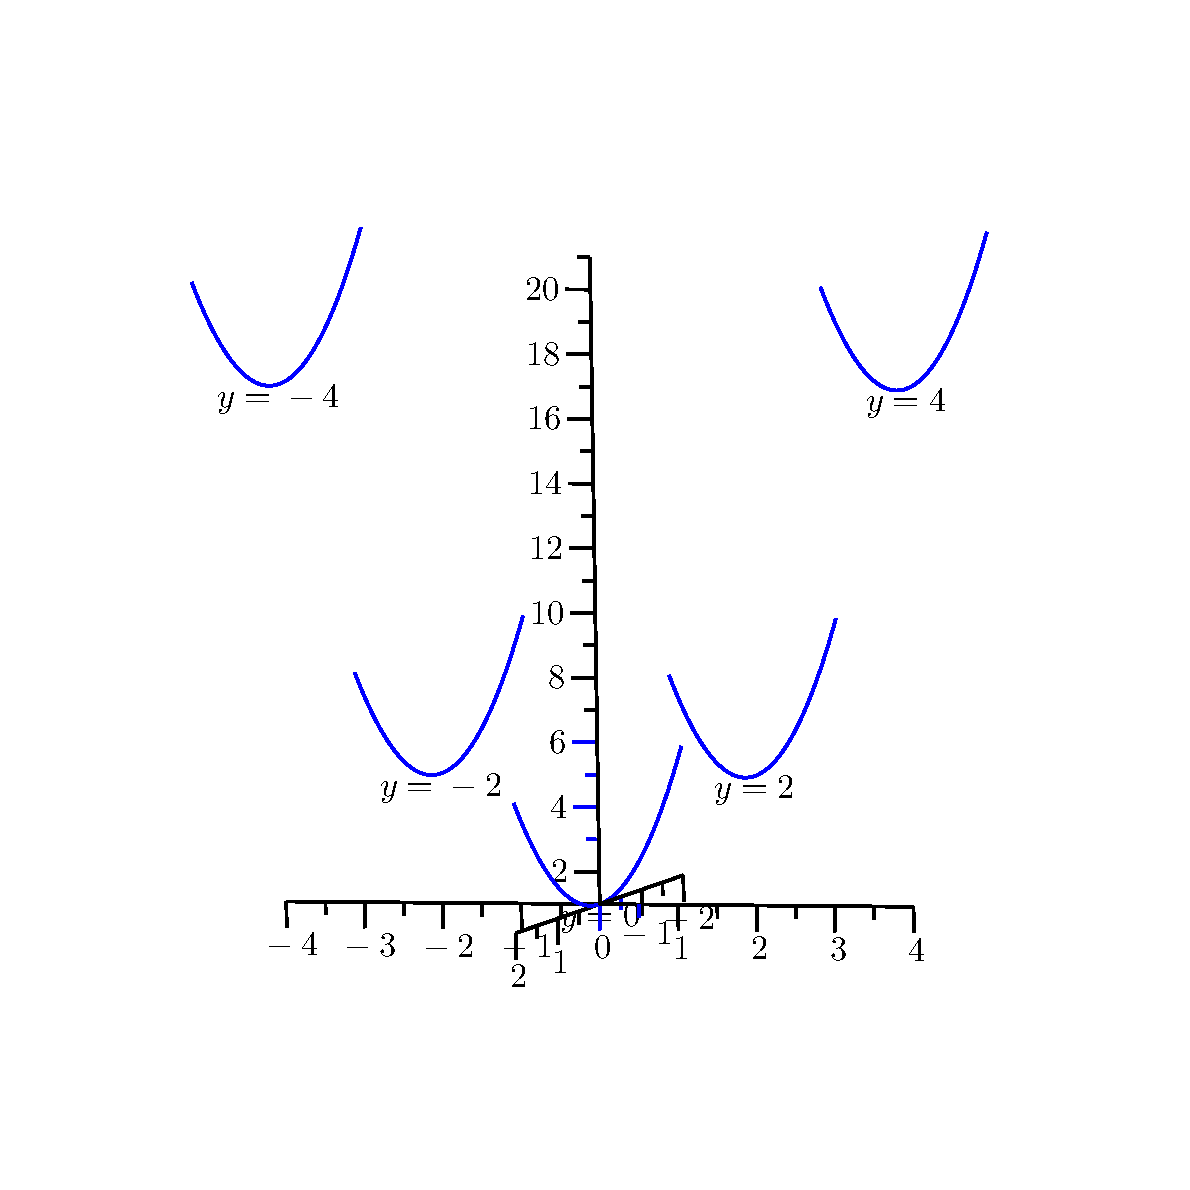
\includegraphics{figures/9_1_Act_6_1}}
%\caption{Traces in the $x$ direction.}
%\label{F:9.1_Act_6_1}
\end{center}
%\end{figure}
 \item The portion of the surface $g$ where $x$ is constant at a value $c$ has the form 
\[g(c,y) = c^2+y^2+1.\]
This is a quadratic parallel to the $yz$-plane with its vertex at the point $(c,0,c^2+1)$, opening in the positive $z$ direction. The indicated traces are shown here %in Figure \ref{F:9.1_Act_6_2}
%\begin{figure}[ht]
\begin{center}
\resizebox{!}{2.0in}{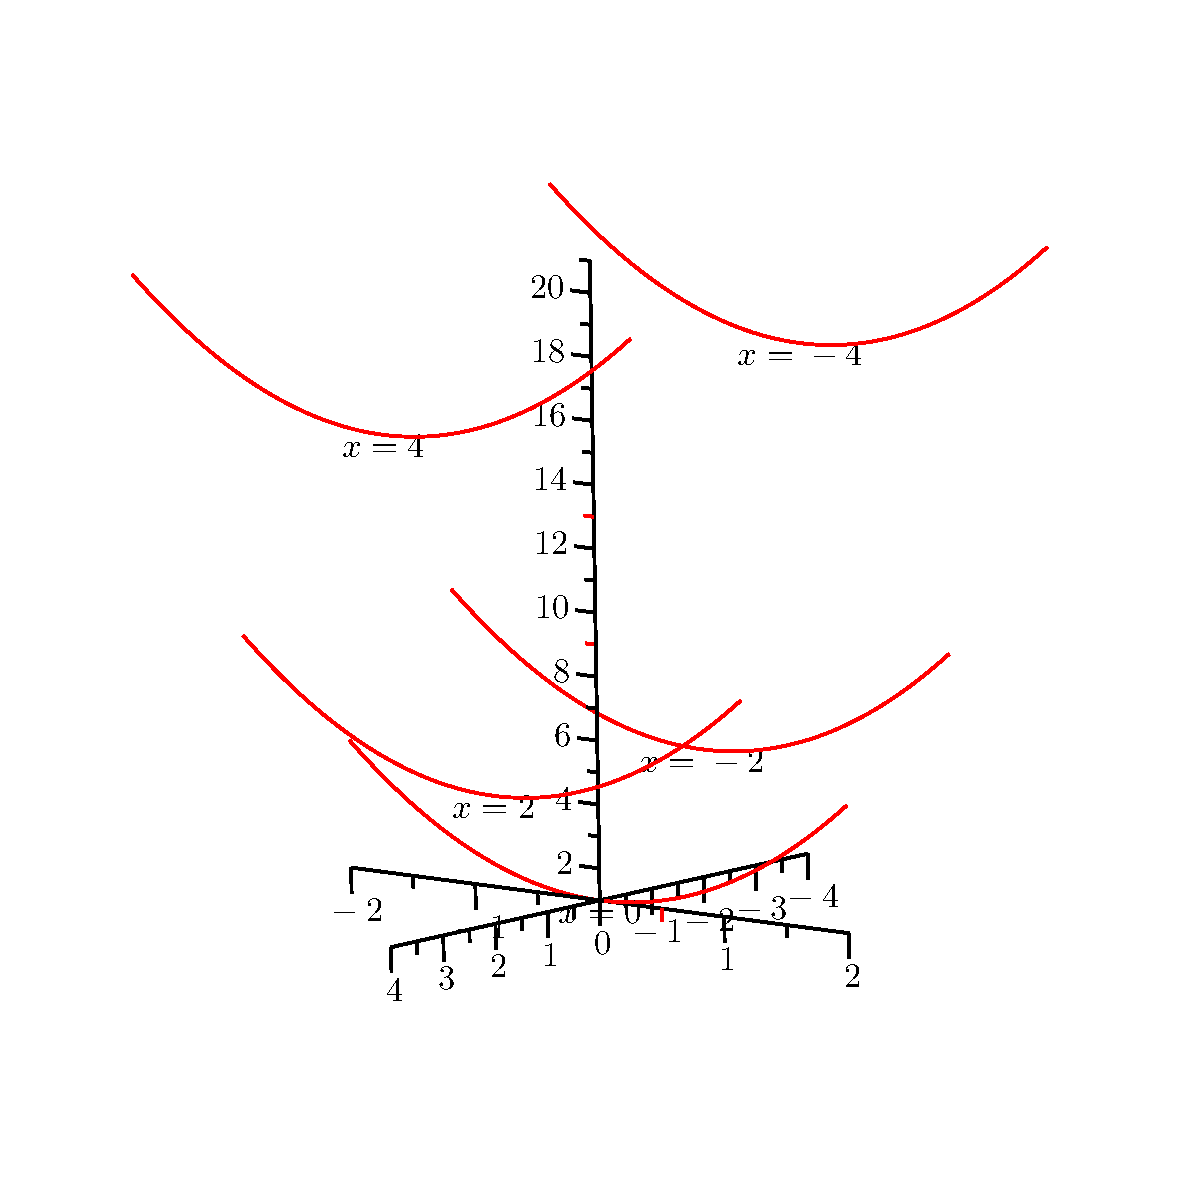
\includegraphics{figures/9_1_Act_6_2}}
%\caption{Traces in the $y$ direction.}
%\label{F:9.1_Act_6_2}
\end{center}
%\end{figure}
\item The traces of $g$ in both directions are parabolas opening in the positive $z$ direction. So the graph of $g$ should look like a bowl with its vertex at the origin, opening in the positive $z$ direction. 
\ea
\end{activitySolution}
\aftera 